\documentclass[10pt]{article}
\setlength{\parskip}{0.25\baselineskip}
\usepackage[margin=1in]{geometry} 
\usepackage{amsmath,amsthm,amssymb, graphicx, multicol, array}
\usepackage[font=small,labelfont=bf]{caption}
\usepackage{float}
\usepackage{bbm}

\newcommand{\supp}{{\text{supp}}} 
\newcommand{\bv}{{\text{BV}}}
\newcommand{\ac}{{\text{AC}}}
\newcommand{\vol}{{\text{Vol}}}

\newenvironment{problem}[2][]{\begin{trivlist}
\item[\hskip \labelsep {\bfseries #1}\hskip \labelsep {\bfseries #2.}]}{\end{trivlist}}

\begin{document}
 
\title{Homework \#8}
\author{Eric Tao\\
Math 123: Homework \#8}
\maketitle

\begin{problem}{Question 1}

Use the data 'HW8\_TwoClass.mat' consisting of data points $\{ x_i \}_{i=1}^n \subset \mathbb{R}^2$ with labels $\{ y_i \}_{i=1}^n$.

(a) Let $F(w,b) = \Vert w \Vert_2^2 + \lambda \sum_{i=1}^n \max(0,1-y_i(w^tx_i +b))$ be the hinge loss. Use MATLAB's optimization function 'fminunc.m' to estimate the hyperplane that minimizes $F(w,b)$ for various choices of $\lambda$. Plot the results of the hyperplanes with the data and discuss.

(b) Let $G(w,b) = \Vert w \Vert_2^2 + \lambda \sum_{i=1}^n \max(0,1-y_i(w^tx_i +b))^2$ be the squared loss. Use MATLAB's optimization function 'fminunc.m' to estimate the hyperplane that minimizes $G(w,b)$ for various choices of $\lambda$. Plot the results of the hyperplanes with the data and discuss.

\end{problem}

\begin{proof}[Solution]

(a)

\begin{center}
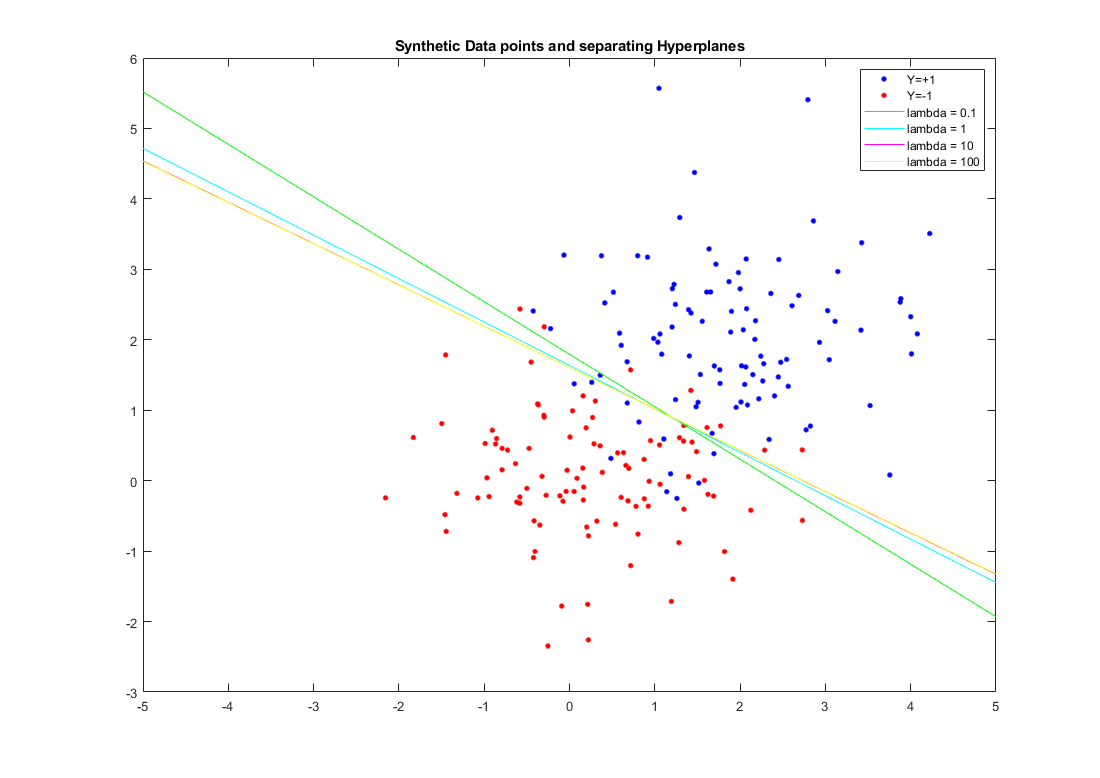
\includegraphics[,scale=0.5]{hinge_loss}
\captionof{figure}{Hinge Loss hyperplanes}
\end{center}

We see that in the center of the scatter plot, where there are ambiguities, the changing angles of the hyperplanes are reflecting the relative priorities of $\lambda$. We can see this with the blue point near $(0.5, 1.5)$. We see that depending on the hyperplane, that point lies on different sides of the hyperplane, depending on if maximizing the margin or if reducing the incorrectness of the classification is more important.

Note that some of these graphs are not easily visible, like the magenta graph, since the parameters vary minimally from $10 \to 100$

(b)

\begin{center}
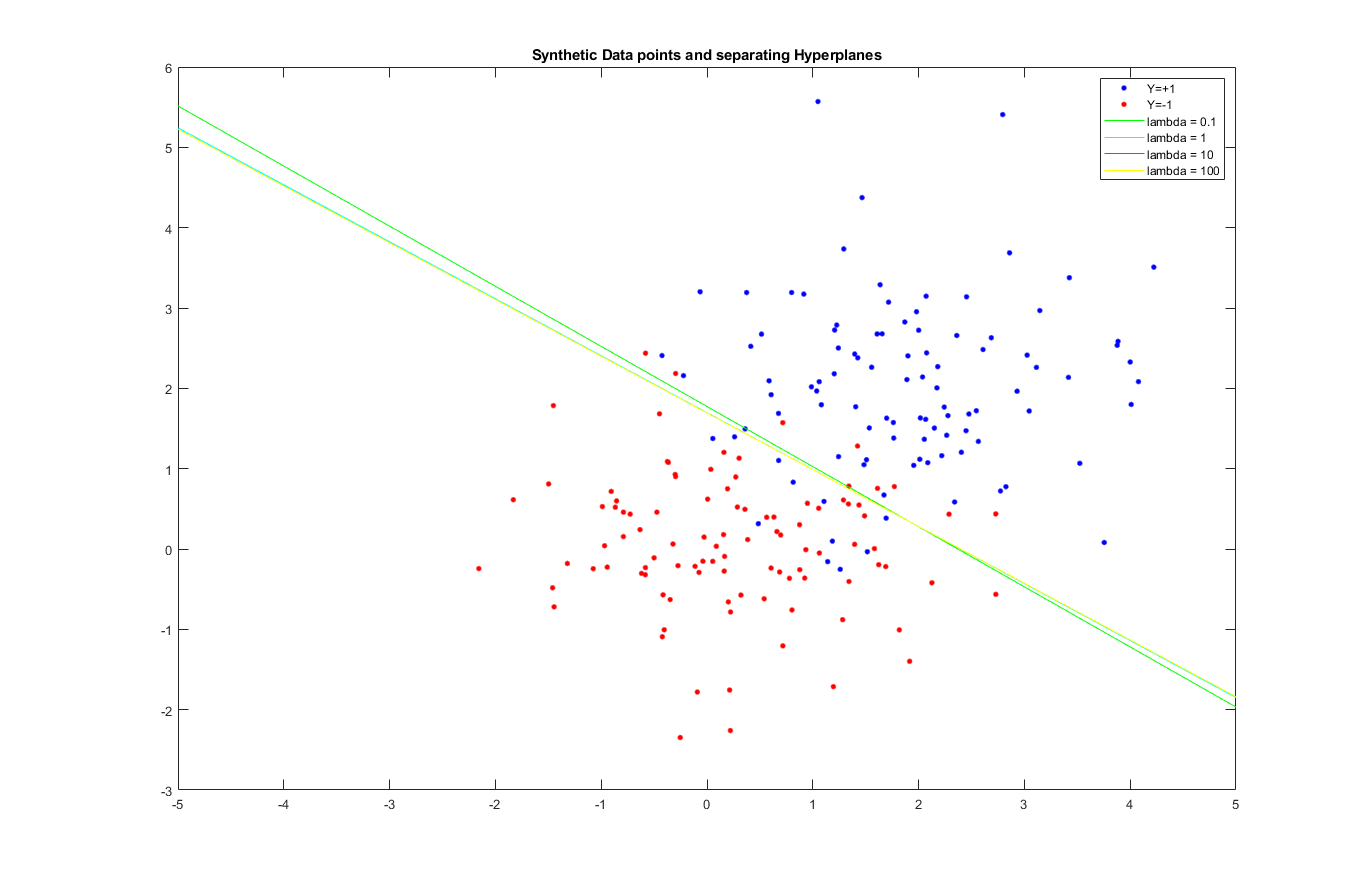
\includegraphics[,scale=0.5]{squared_loss}
\captionof{figure}{Squared Loss hyperplanes}
\end{center}

In a similar fashion, we see the same behavior as in the linear hinge loss case. However, we also note that in the squared loss case, the variation in the optimal hyperplane varies less with the change in lambda. This is due to the squared weight on the incorrect portion.



\end{proof}

\begin{problem}{Question 2}

Suppose that we have data points $\{(x_i, y_i)\}_{i=1}^n$ with $x_i \in \mathbb{R}^D$, and $y_i \in \{ -1,1\}$, with the data classes being linear separable, that is, there exists a hyperplane such that all points with label $-1$ are on one side and all points with label $1$ are on the other.

(a) Phrase the linear separability condition mathematically in terms of the parameters of the hyperplane.

(b) Prove that if there exists a single hyperplane, then there are infinitely many.

(c) Let $F(w,b) = \Vert w \Vert_2^2 + \lambda \sum_{i=1}^n \max(0,1-y_i(w^tx_i +b))$ be the soft-margin hinge loss with regularization parameter $\lambda$. Describe the resultant hyperplanes as $\lambda \to 0$ and for $\lambda \to +\infty$.

(d) Suppose for a fixed $\lambda$, $(w^*, b^*)$ are the minimizing parameters. How do we use these parameters to classify a new point $x_{\text{test}}$?

\end{problem}

\begin{proof}[Solution]

(a)

Suppose the hyperplane is given by, for a (row) vector $w \in \mathbb{R}^D$, a value $b \in \mathbb{R}$, and a (column) input $x \in \mathbb{R}^D$ the expression:

$$ H = wx + b $$

Then, we say that the data classes are linearly separable, if there exists $w, b$ such that for all $x_i$, we have that $\text{sgn}( w x_i + b) = y_i$, where we take sgn as the sign function that sends positive numbers to $+1$ and negative numbers to $-1$, and 0 to 0.

(b)

Suppose we have $(w,b)$ such that the hyperplane linearly separates our data points, $X$. Viewing the hyperplane as $H(x) = wx + b = 0$, since this is a continous function, and $\{ 0 \}$ is closed, the hyperplane is a closed set. Further, since our data points are strictly a collection of singletons, $X$ is closed, and further, compact. Lastly, we must have that our hyperplane is disjoint with our data set, as no data points can lie in our hyperplane for the decision based on the sign to be valid.

Since $\mathbb{R}^D$ is a metric space, there exists $\delta > 0$ such that the minimum distance between $X, H$ is at least $\delta$. I will use this without proof, but essentially, if we have a closed set, compact set, disjoint, and we suppose that there exists $x_n \in X, y_n \in Y$ such that $d(x_n, y_n) \to 0$, then they must converge to the same point, a contradiction with the disjointness. Then, choose any $0 < \epsilon < \delta$. Consider the related, parallel hyperplane

$$ H' = wx + b + \epsilon$$

By definition, this is a hyperplane that is $\epsilon$ away from $H$. In particular, because we have that $\delta$ is the smallest distance between $H$ and any point, and $\epsilon$ is less than that, the relative positions of any point $x_i$, and $H'$ cannot change from how they are oriented with respect to $H$. Since $(0,\delta)$ has the cardinality of the continuum, and we may choose any $\epsilon$ in here, this is an (uncountably) infinite family of separating hyperplanes.

(c)

Assume that this is the only loss function we use, and we do not have any hard conditions on the hyperplane. If we take $\lambda \to 0$, this implies that the main condition on the hyperplane is that $\Vert w \Vert_2^2$ is as small as possible, which prioritizes the margin on the sets. However, as $\lambda$ gets too small, the loss function that penalizes hyperplanes that do not properly separate into the two classes becomes small, and so we permit hyperplanes with $w = 0$, and $b$ such that the hyperplane is arbitrarily far away from our data points.

Now, suppose instead that $\lambda \to \infty$. In such a case, the loss function penalizing incorrect classification of points becomes large, and thus we weight towards hyperplanes that correctly classify the data classes potentially at the cost of reducing the margin between the classes and the hyperplane.

(d)

Here, we use the same idea as the linear separability condition. That is, we compute:

$$ \text{sgn}( w^*x_{\text{test}} + b^*)$$

If this is equal to $+1$, then we classify it as belonging to the $y = +1$. If it is equal to $-1$ then we classify it as belong to the label $y = -1$. If it lies on the hyperplane, we have ambiguity.

\end{proof}



\end{document}